\section{Verhalten von Bahnkurven in 2D} \label{poinbendix:section:nullklinen}

Das Verhalten von Bahnkurven in 2D kann anhand von verschiedenen Methoden analysiert werden.
Dabei gehen wir immer von $r$-fach differenzierbaren dynamischen Systemen aus, welche also stetige Bahnkurven hervorbringen.
Die Bahnen in diesen Systemen sind dann zu einem gewissen Grad vorhersagbar durch die Analyse der Nullklinen.
Ein Beispiel dazu findet sich im nächsten Abschnitt \ref{poinbendix:subsection:nullklinen}.
In einem zweiten Abschnitt \ref{poinbendix:subsection:limesmengen} werden dann die sogenannten Limesmengen eingeführt, welche den Kern des Satzes von Poincaré-Bendixson bilden.
\index{Limesmengen}%

\subsection{Nullklinen} \label{poinbendix:subsection:nullklinen}

Die Punkte, bei denen die Ableitungen entlang einer Koordinatenachse null
werden (z.~B.: $\dot{x}=0$), befinden sich auf Kurven, welche \emph{Nullklinen} genannt werden.
\index{Nullkline}%
Somit werden Nullklinen in 2D immer von einem vertikalen ($x$-Nullkline) oder einem horizontalen ($y$-Nullkline) Fluss durchflossen.
Daraus folgt, dass Schnittpunkte zweier Nullklinen Nullstellen sind (in 2D).
Alle Ableitungen werden also null ($\dot{x}=\dot{y}=0$) und Bahnkurven, welche zu diesen Punkten kommen, enden sofort.

Die Nullklinen unterteilen die Ebene in unterschiedliche Sektoren, welche jeweils eine bestimmte Flussrichtung haben.
Da das dynamische System stetig ist, gibt es keine Sprünge in den Nullklinen.

Dies bedeutet, dass eine $x$-Nullkline in einem Abschnitt zwischen zwei Nullstellen zum Beispiel immer von oben nach unten durchflossen wird ($\dot{y} < 0$).
Die vertikale Flussgeschwindigkeit kann dabei variieren.
Nachdem eine Nullstelle erreicht wird, kann die Flussrichtung wechseln.

Wie man Anhand von Nullklinen mögliche Bahnkurven vorhersagen kann, wird anhand des folgenden Beispiels gezeigt.

\begin{beispiel} \label{poinbendix:beispiel:nullklinen}

Für das dynamische System
\begin{align*}
    \dot{x} &= y - x^2 \\
    \dot{y} &= x - y^3
\end{align*}
können durch Nullsetzen die $x$- und $y$-Nullklinen als Funktionen
\begin{align*}
    y_x(x) &= x^2 \\
    y_y(x) &= \sqrt[3]{x}
\end{align*}
gefunden werden.
Durch Gleichsetzen der beiden Nullklinen
\begin{align*}
    x^2 &= \sqrt[3]{x} \\
    x^6 &= x
\end{align*}
erhält man dann zwei Nullstellen an den Punkten $(0, 0)$ und $(1, 1)$.

In Abbildung \ref{poinbendix:fig:nullklinen} sieht man, wie sich die $x$-Nullkline (rot) und die $y$-Nullkline an den beiden Nullstellen kreuzen.
Es ergeben sich fünf Regionen mit unterschiedlicher Flussrichtung.

Wenn man sich diese Regionen um die Nullpunkte genauer anschaut, kann man schon eine ungefähre Vorstellung von möglichen Bahnkurven bekommen (siehe die beiden vergrösserten Ausschnitte in Abbildung \ref{poinbendix:fig:nullklinen}).
Zur Erinnerung, die Ableitungen können nur auf den Nullklinen ihre Richtung wechseln.
Daraus folgt, dass ein einzelner Punkt pro Region genügt, um den (generellen) Fluss in der gesamten Region vorherzusagen.

Nehmen wir den Punkt $(-2, 0)$, welcher in der Region links liegt.
Dann erhalten wir
\[
\renewcommand{\arraycolsep}{3pt}
\begin{array}{rcccl}
\dot{x} &=& y-x^2 &=&-4 \\
\dot{y} &=& x-y^3 &=&-2.
\end{array}
\]
Somit gehen die Bahnkurven in der linken Region nach unten links, wobei sie durch die $y$-Nullkline $y_y(x) = \sqrt[3]{x}$ nach unten beschränkt werden.

Mit derselben Methode können auch die anderen 4 Regionen analysiert werden.
\end{beispiel}

\begin{figure}
    \centering
    \begin{tikzpicture}[>=stealth, scale=1.5]
  
  % Draw axes
  \draw[thick, black, ->] (-2,0) -- (2,0); % Horizontal axis
  \draw[thick, black, ->] (0,-2) -- (0,2); % Vertical axis
  
  % Axis labels
  \node[above] at (0,2) {$\dot{y} = 0$};
  \node[right] at (2,0) {$\dot{x} = 0$};
  
  % Define colors for each quadrant
  \colorlet{q1color}{red}
  \colorlet{q2color}{blue}
  \colorlet{q3color}{green}
  \colorlet{q4color}{orange}

  % Clockwise arrows in each quadrant, at 45° angles with unique colors
  % First quadrant: down-right (southeast)
  \draw[q1color, ->] (0.5,1.5) -- (1.5,0.5);
  \node[above, right, q1color] at (1,1) {$\dot{x} > 0, \dot{y} < 0$};
  
  % Second quadrant: down-left (southwest)
  \draw[q2color, ->] (1.5,-0.5) -- (0.5,-1.5);
  \node[below, right, q2color] at (1,-1) {$\dot{x} < 0, \dot{y} < 0$};
  
  % Third quadrant: up-left (northwest)
  \draw[q3color, ->] (-0.5,-1.5) -- (-1.5,-0.5);
  \node[below, left, q3color] at (-1,-1) {$\dot{x} < 0, \dot{y} > 0$};
  
  % Fourth quadrant: up-right (northeast)
  \draw[q4color, ->] (-1.5,0.5) -- (-0.5,1.5);
  \node[above, left, q4color] at (-1,1) {$\dot{x} > 0, \dot{y} > 0$};
  
\end{tikzpicture}

    \caption{Darstellung der Nullklinen und der Flussrichtungen aus Beispiel \ref{poinbendix:beispiel:nullklinen}. Die $x$-Nullkline ist rot und die $y$-Nullkline blau eingezeichnet. Darstellung von Nicolas Tobler.}
    \label{poinbendix:fig:nullklinen}
\end{figure}

\subsection{Limesmengen} \label{poinbendix:subsection:limesmengen}

Limesmengen beinhalten alle Punkte, welchen sich Bahnkurven unendlich oft annähern.
\index{Limesmengen}%
Dies können einzelne Punkte sein, periodische Bahnen, oder Kombinationen davon.
Dabei startet man bei einem beliebigen Punkt $p \in M$ und schaut sich das Verhalten in positiver und negativer Zeit an.

Formell betrachtet bestehen die Limesmengen aus sogenannten Häuffungspunkten, also allen Punkten, denen die Bahn beliebig nahe kommt.
\begin{definition}[Häuffungspunkte]
\index{Häuffungspunkt}%
\label{poinbendix:def:limesmengen}
$q$ ist ein Häufungspunkt der Bahn $\Phi_t(p)$, wenn es für jedes $\epsilon > 0$ und jedes $N > 0$ einen Zeitpunkt $t > N$ gibt, sodass der Abstand $d(\Phi_t(p),q) < \epsilon$ ist.
\end{definition}

Ist die Bahnkurve periodisch, so werden die Häuffungspunkte immer wieder nach diskreten Zeitpunkten $t_i$ erreicht.
\begin{definition}[Limesmengen]
\label{poinbendix:def:limesmengen}
\index{Limesmenge}%
Die Alpha- und Omega-Limesmengen
\index{Alpha-Limesmenge}%
\index{Omega-Limesmenge}%
\begin{align*}
    \alpha(p) &= \{q\in M; \; \Phi_{t_i}(p) \to q \; \text{für eine Sequenz} \; t_i \to -\infty\} \\
    \omega(p) &= \{q\in M; \; \Phi_{t_i}(p) \to q \; \text{für eine Sequenz} \; t_i \to \infty\}
\end{align*}
beschreiben das Verhalten eines dynamischen Systems $\Phi_{t_i}(p)$ nach einer gegen Unendlich strebenden Folge von Zeitpunkten $t_i$.
\end{definition}

Vereinfacht gesagt, beschreibt $\alpha(p)$, von wo aus die Bahnkurve den Punkt $p$ erreicht und $\omega(p)$ wohin sich die Bahnkurve danach fortbewegt\footnote{Alpha und Omega sind der erste, respektive letzte Buchstabe im griechischen Alphabet, weshalb die Benennung der Limesmengen intuitiv Sinn ergibt.}.

\begin{beispiel} \label{poinbendix:beispiel:1dlimesmengen}
Schauen wir uns die einfache, eindimensionale Differenzialgleichung
\begin{equation*}
    \dot{x} = \sin x,
\end{equation*}
mit einem Startpunkt von $p = \frac{\pi}{2}$ an.
Am Punkt $p$ haben wir eine positive Ableitung ($\dot{x} = 1$), und der Punkt wird eingeschlossen von zwei Nullstellen $0$ und $\pi$.
Daraus folgt, dass beide Limesmengen auf die Nullstellen fallen $\alpha(p) = 0$ und $\omega(p) = \pi$.
Eine Darstellung dieses Beispiels findet sich in Abbildung \ref{poinbendix:fig:limesmenge}.
\begin{figure}
    \centering
    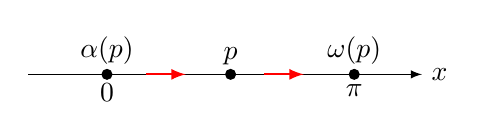
\begin{tikzpicture}[>=latex]
  \draw[->] (-1,0) -- (4,0) node[right] {$x$};
  \fill (0,0) circle (2pt) node[below] {$0$} node[above] {$\alpha(p)$};
  \fill (3.14,0) circle (2pt) node[below] {$\pi$} node[above] {$\omega(p)$};
  \fill (1.57,0) circle (2pt) node[above] {$p$};
  \draw[red,->,thick] (0.5,0) -- (1,0);
  \draw[red,->,thick] (2,0) -- (2.5,0);
\end{tikzpicture}

    \caption{Darstellung der Limesmengen aus Beispiel \ref{poinbendix:beispiel:1dlimesmengen}.}
    \label{poinbendix:fig:limesmenge}
\end{figure}
\end{beispiel}
